\section{From automaton to regular expression}

Suppose for simplicity the initial state $i$ is unique, and no arc enters in it; similarly the final state $t$ is unique and without outgoing arcs. 
Every state other than $i$ and $t$ is called internal. 
We construct an equivalent automaton, termed generalized finite automaton,  that allows arc labels to be also regular languages. 
Eliminate the internal nodes one by one, and after each elimination add one or more compensation arcs to preserve the equivalence of the automaton.
Such new arcs are labeled by regular expressions.
At the end only the nodes $i$ and $t$ are left, with only one arc from $i$ to $t$. 
The regular expression that labels such an arc generates the complete language recognized by the original finite automaton. 

The elimination order is not relevant.
However, different orders may generate different regular expressions, all equivalent to one another but of different complexity.
\begin{example}
    Consider the following automaton: 
    \begin{figure}[H]
        \centering
        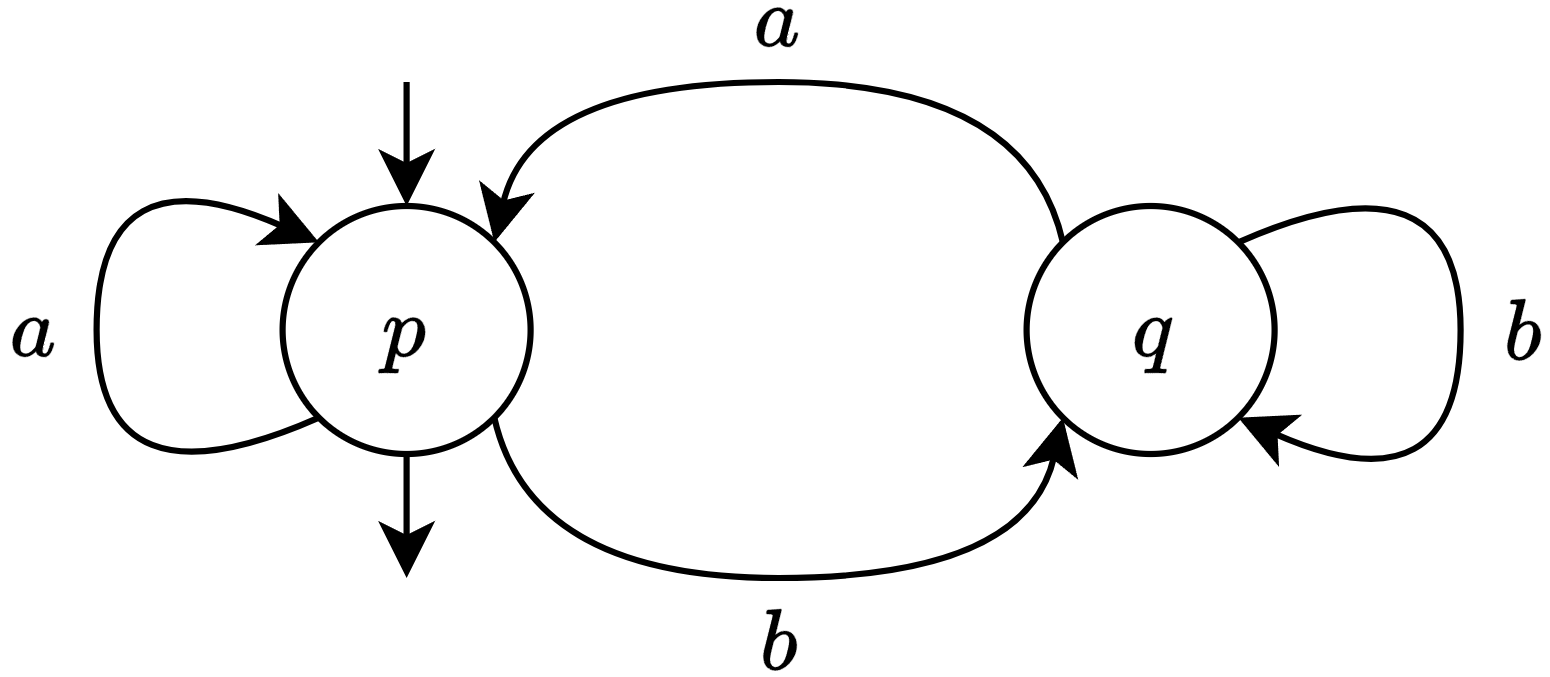
\includegraphics[width=0.25\linewidth]{images/br1.png}
    \end{figure}
    We have to normalize it to obtain the initial state and the final state, obtaining: 
    \begin{figure}[H]
        \centering
        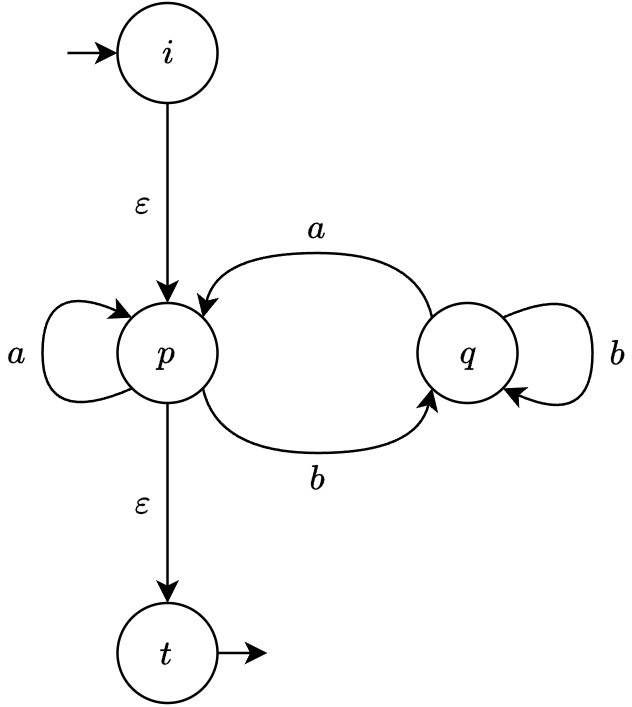
\includegraphics[width=0.25\linewidth]{images/br2.png}
    \end{figure}
    Finally, we can apply the Brzozowski and McCluskey method to the normalized automata.
    We do this in three steps that consist in: 
    \begin{enumerate}
        \item Eliminate the node $q$, replacing it with the regular expression $bb^{*}a$.
        \item Merge the two cycles on node $p$ with the choice operator, obtaining: $a|bb^{*}a=b^{*}a$. 
        \item Remove the node $p$ by replacing the label of the arc with $(b^{*}a)^{*}$
    \end{enumerate}
    \begin{figure}[H]
        \centering
        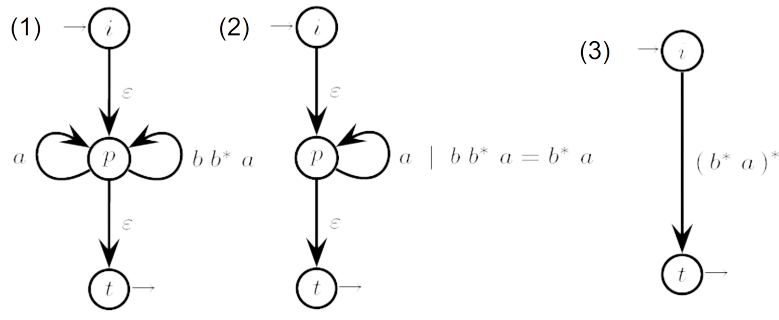
\includegraphics[width=0.5\linewidth]{images/br3.png}
    \end{figure}
\end{example}